\scanpage{176}
% archive sheet number: 175
\[
\mathscr{E}xt^p(F,G)
\]

\[
\mathscr{E}xt^{\unsure{p|q|n}}(i_!(F),G)\simeq
\unsure{\mathscr{E}|\mathrm E}xt^p(F,\mathbb R i^!(G))
\]

\[
\mathscr{E}xt^*(F,\mathbb R i^!(G))\unsure{\Leftarrow|\ne|=}E_2^{pq}=\mathscr{E}xt^p(F,\mathbb R^qi^!(G))
\]

\diagram{\begin{tikzcd}[ampersand replacement=\&,column sep=0.4em]
Y \& \unsure{\longleftrightarrow|\longleftarrow|\hookrightarrow} \& X
\end{tikzcd}}

\[
\mathscr{E}xt^p(F,\underset{\rule{.5pt}{.4em}\rule{3em}{.5pt}\rule{.5pt}{.4em}}{\mathbb R^qi^!G})
\]

\[
\mathscr{E}xt^p
\]

\figure{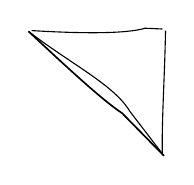
\begin{tikzpicture}[x=1cm,y=1cm]
\draw (0.04,1.59) .. controls (.7,1.55) and (1.25,1.55) .. (1.48,1.62) -- (1.70,1.61);
\draw (1.74,1.59) .. controls (1.73,1.0) and (1.69,.45) .. (1.70,.01);
\draw[semithick] (0,1.58) .. controls (.45,1.16) and (.92,.72) .. (1.19,.54) -- (1.72,0);
\draw (0,1.58) .. controls (.53,1.17) and (1.09,.90) .. (1.29,.56) -- (1.72,0);
\end{tikzpicture}}

\diagram{\scriptsize\setlength{\arraycolsep}{1.6pt}
$\begin{array}{c@{}c@{\;}c@{}c@{}c@{\quad}c@{}c@{\quad}c@{}cc}
\unsure{\leq d|2d} & & \leq d-1 & & \leq d-2 & & & & 0 &\\
\mathscr{E}xt^0, & \mathscr{E}xt^1 & \mathscr{E}xt^2 & / &
\mathscr{E}xt^3\;\mathscr{E}xt^4 & / & & / & \mathscr{E}xt^{2d-1}, & \mathscr{E}xt^{2d}
\end{array}$}

\[
H^p(X,\mathscr{E}xt^q\qquad
\deleted{H^{\unsure{n|q}}}\ H^{\unsure{n|2d}}(X,\mathscr{E}xt^0)+H^{n-1}\mathscr{E}xt^1,\ \unsure{.|\,}
\]

\figure{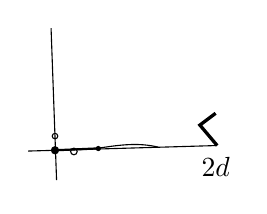
\begin{tikzpicture}[x=1cm,y=1cm]
\draw (-.05,1.55) -- (.02,-.38);
\draw (-.34,-.01) -- (2.05,.06);
\draw[thick] (0,0) -- (.58,.025);
\draw (.54,.025) .. controls (.83,.07) and (1.06,.10) .. (1.31,.04);
\fill (0,0) circle (1.5pt); \draw (.0,.18) circle (1pt); \draw (.24,-.015) circle (1.2pt);
\fill (.55,.022) circle (.95pt);
\draw[very thick] (2.06,.06) -- (1.84,.32) -- (2.04,.47);
\node[below] at (2.04,.04) {$2d$};
\end{tikzpicture}}

\[
p\leq \qquad
\begin{array}{ccc}
 & n-1\unsure{.|\,}\leq2(d-1)&n-3\leq2(d-2)\\
n\leq2d & \deleted{\unsure{n-1|n+1}\leq2d-1}&\\
 & n-2\leq2(d-1)&n-4\leq2(d-2)
\end{array}
\]

\[
\deleted{\mathrm{Ext}^*(F,G)\simeq}\qquad \underline{2d-1}
\]

\figure{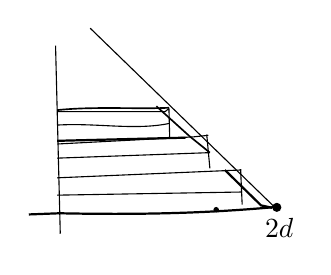
\begin{tikzpicture}[x=1cm,y=1cm]
\draw (-.02,2.13) -- (.04,-.26);
\draw[thick] (-.36,-.015) -- (.03,0) .. controls (1.25,-.025) and (2.06,.015) .. (2.78,.08);
\draw (.42,2.35) -- (2.76,.08);
\draw[semithick] (.0,1.31) .. controls (.47,1.36) and (1.03,1.32) .. (1.42,1.34);
\draw (.00,1.29) -- (1.37,1.29) -- (1.42,1.33) -- (1.43,.95);
\draw (.0,1.12) .. controls (.51,1.15) and (.98,1.05) .. (1.42,1.14);
\draw[thick] (.0,.92) -- (1.63,.96); \draw (.01,.88) -- (1.73,.97) -- (1.92,.99);
\draw (.0,.70) -- (1.94,.77); \draw (1.90,1) -- (1.94,.57);
\draw (.0,.45) -- (2.34,.55); \draw (2.33,.56) -- (2.35,.11);
\draw (.0,.23) -- (2.35,.27);
\draw[semithick] (1.26,1.36) -- (1.68,.98) -- (1.94,.77);
\draw[thick] (2.13,.55) -- (2.59,.10) -- (2.73,.07);
\fill (2.02,.045) circle (1pt); \fill (2.79,.075) circle (1.65pt);
\node[below] at (2.82,.06) {$2d$};
\end{tikzpicture}}

\[
\mathbb R\mathscr{H}om(F,\deleted{\unsure{D|G}}G)\simeq
\mathbb R\mathscr{H}om(F\otimes DG,K_X)
\]

\[
\mathrm{Ext}^{p+q}(X;F,G)\Leftarrow E_2^{pq}=\mathrm{Ext}^p(X;\mathrm{Ext}^{-q}(X;G,A_X),A_X)
\]

\[
\mathrm{Ext}^{2d}(X;F,G)
\]

\figure{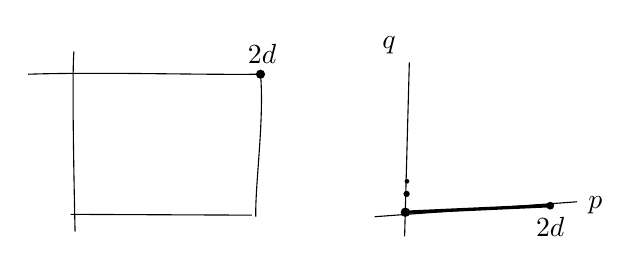
\begin{tikzpicture}[x=1cm,y=1cm]
\draw (0,2.12) .. controls (-.025,1.81) and (.0,.49) .. (.015,-.17);
\draw (-.58,1.83) .. controls (.35,1.86) and (1.57,1.82) .. (2.37,1.83);
\draw (2.37,1.83) .. controls (2.42,1.26) and (2.30,.43) .. (2.31,.02);
\draw (-.04,.05) -- (2.26,.04); \fill (2.37,1.83) circle (1.65pt);
\node[above] at (2.39,1.84) {$2d$};
\begin{scope}[xshift=4.2cm]
\draw (.06,1.98) -- (0,-.23); \draw (-.38,.02) -- (2.19,.21);
\draw[very thick] (.01,.077) -- (1.85,.16); \fill (.01,.077) circle (1.7pt);
\fill (.025,.31) circle (1.15pt); \fill (.03,.47) circle (.85pt); \fill (1.85,.16) circle (1.4pt);
\node[above left] at (.01,1.96) {$q$}; \node[right] at (2.21,.16) {$p$}; \node[below] at (1.85,.135) {$2d$};
\end{scope}
\end{tikzpicture}}

\[
\mathrm{Ext}^*(X;F,A_X)\Leftarrow \deleted{\unsure{E|H}}H^p(X,\mathscr{E}xt^q(F,A_X))\qquad{}^{2(d}
\]

\[
H^{2d}(X,
\]

\figure{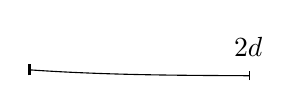
\begin{tikzpicture}[x=1cm,y=1cm]
\draw (0,0) .. controls (1,-.07) and (2,-.07) .. (2.80,-.075);
\draw[very thick] (0,-.07) -- (0,.07); \draw (2.8,-.13) -- (2.8,-.01);
\node[above] at (2.78,.05) {$2d$};
\end{tikzpicture}}
